\documentclass[conference]{IEEEtran}
\IEEEoverridecommandlockouts
% The preceding line is only needed to identify funding in the first footnote. If that is unneeded, please comment it out.
\usepackage{cite}
\usepackage{amsmath,amssymb,amsfonts}
\usepackage{algorithmic}
\usepackage{graphicx}
\usepackage{textcomp}
\usepackage{xcolor}
\usepackage[export]{adjustbox}
\graphicspath{ {./images/} }
\def\BibTeX{{\rm B\kern-.05em{\sc i\kern-.025em b}\kern-.08em
    T\kern-.1667em\lower.7ex\hbox{E}\kern-.125emX}}
\begin{document}

\title{Test Your Limits With TRex traffic generator 
\thanks{Cisco systems}
}



\author{\IEEEauthorblockN{Hanoch Haim}
\textit{Cisco systems}\\
}

\maketitle

\begin{abstract}
Performance measurement tools are an integral part of network testing. 
There is no shortage of open source tools for network performance
testing in the Linux world. 
To enumerate a few popular tools in the Linux world: Netperf, iperf, Linux kernel based pktgen.
These tools tend to fall into two categories:
\begin{itemize}
  \item  Stateless packet shooting such as the linux kernel pktgen traffic generator 
  \item Stateful client-server tools such as netperf and iperf. 
\end{itemize}  
When very high performance network performance testing is required (quantified as
many 10s of Gigabits per second/100MPPS and/or hundreds of thousands of flows) or more advanced functionality (e.g. realistic) is required the
linux classical tools are insufficient. Most organizations
will opt for very expensive commercial tools such as Ixia, Spirent. 
In this paper we will introduce TRex a high performance realistic traffic generator
and illustrate sample stateless and stateful use cases that apply to testing
Linux networking. We will also discuss its design and tricks that help us
achieve such high performance.
\end{abstract}

\begin{IEEEkeywords}
tcp, performance, scale,realistic traffic generation 
\end{IEEEkeywords}

\section{Introduction}

TRex \cite{b1} is an advanced traffic generator, it has the following interesting features:

\begin{itemize}
\item It leverages COTS x86/ARM servers and Physical NICs (Intel, Mellanox etc) for high scale 
\item Can support linux driver or paravirtual (e.g. virtio) for low scale advance feature 
\item  It can serve both Stateless and Stateful traffic generation.
  tcp stack for stateful traffic and emulation layer to simulate L7 applications
\item It outperforms all of iperf, netperf and pktgen 
   \begin{itemize}
    \item It can generate upto 200gbps/100mpps advance traffic pattern and millions of real
      world tcp/udp flows.
    \item High connection rate - order of Millions of Connection/s (CPS)
  \end{itemize}
\item It is extensible
\begin{itemize}
    \item Emulate L7 application (on top of TCP/IP),
       e.g. HTTP/HTTPS/Citrix using a programable language
    \item Ability to change fields in the L7 application - for example,
      change HTTP User-Agent field
\end{itemize}
\item Support routing protocols like BGP/OSPF/RIP using BIRD \cite{b4}
\item Support high scale client simulation protocols (arp.ipv6-nd,dhcp,802.1x,icmp) 
\end{itemize}
Although TRex is implemented on top of DPDK, a lot of the issues we had
to deal with when writing the tool apply equally to scaling Linux networking;
we share our experiences in that regard and hope to inspire some
of the techniques to be adopted in Linux.

\section{Software design high level}

\begin{figure}[h]
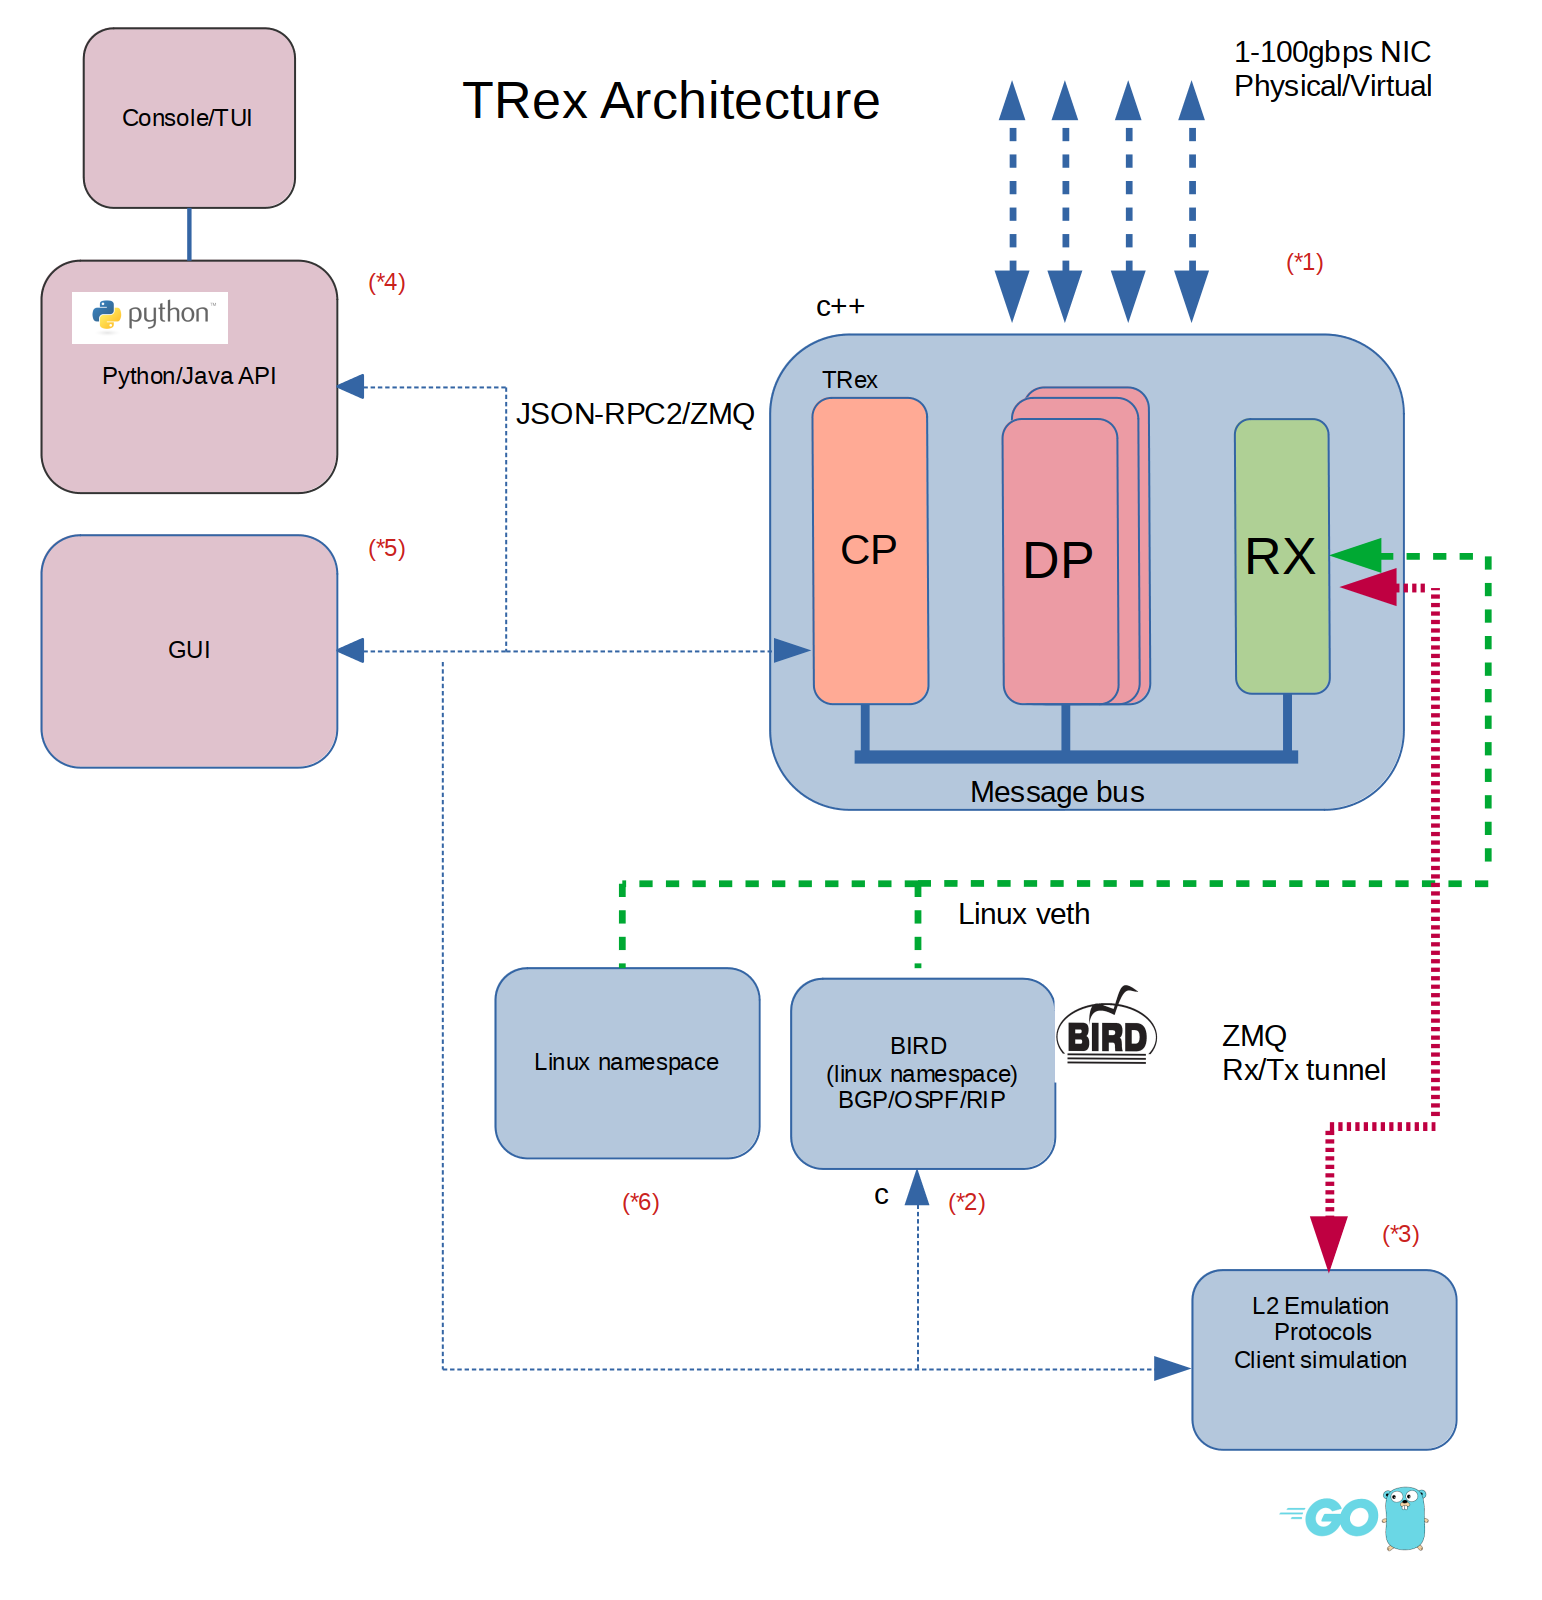
\includegraphics[width=0.4
\textwidth, center]{trex_arch_2.png}
\caption{architecture}
\label{fig:arch}
\end{figure}

Figure \ref{fig:arch} presents the main processes. TRex server (*1) is a multi-threaded process, each thread is pinned to a core and works in 
event driven fashion using a user-space scheduler with a few hierarchy. There is one control-plane (CP) thread that handle the RPC over ZMQ requests and maintenance tasks. 
The RX thread responsible to handle the low latency traffic for accurate latency measurement. This thread is usually in very low CPU. 
The DP threads are generating the traffic using and interact with DPDK to transmit/receive traffic via PMD queues. The number of DP threads can be scale up as the number of Tx/Rx queues. 
There is almost no sharing data structure and no locks to get to best performance. Any information is moved between the threads using a messaging bus which 
is a shared rings (DP$\rightarrow$CP, CP$\rightarrow$DP, Rx$\rightarrow$DP, RX$\rightarrow$CP).
There is minimum system call to the kernel (only when required for example with PF\\\_PACKET driver)
(*4) is a Python wrapper to the JSON-RPC2 API over ZMQ so it would be easy automation (e.g. load a profile, get statistics etc)
on top of Python API there is a Console that can simplify the way to work with the API. 
(*5) is the GUI process that written in Java that works directly with the JSON-RPC2 and supports only the Stateless mode.
(*2) is a BIRD \cite{b4} process that works inside a linux namespace and connected to TRex via a programmable veths. Inside TRex RX thread there is a Switch that forward packets to/from the veth related to the linux namespace. BIRD is used to simulate routing protocols like BGP/OSPF/RIP.
(*6) and (*3) is used for simulating clients slow-path protocols like ARP/IPV6-ND/IGMP/MLD/802.1x/DHCP/DHCPv6 while TRex server is for the fast-path high speed TCP/UDP

\begin{figure}[h]
  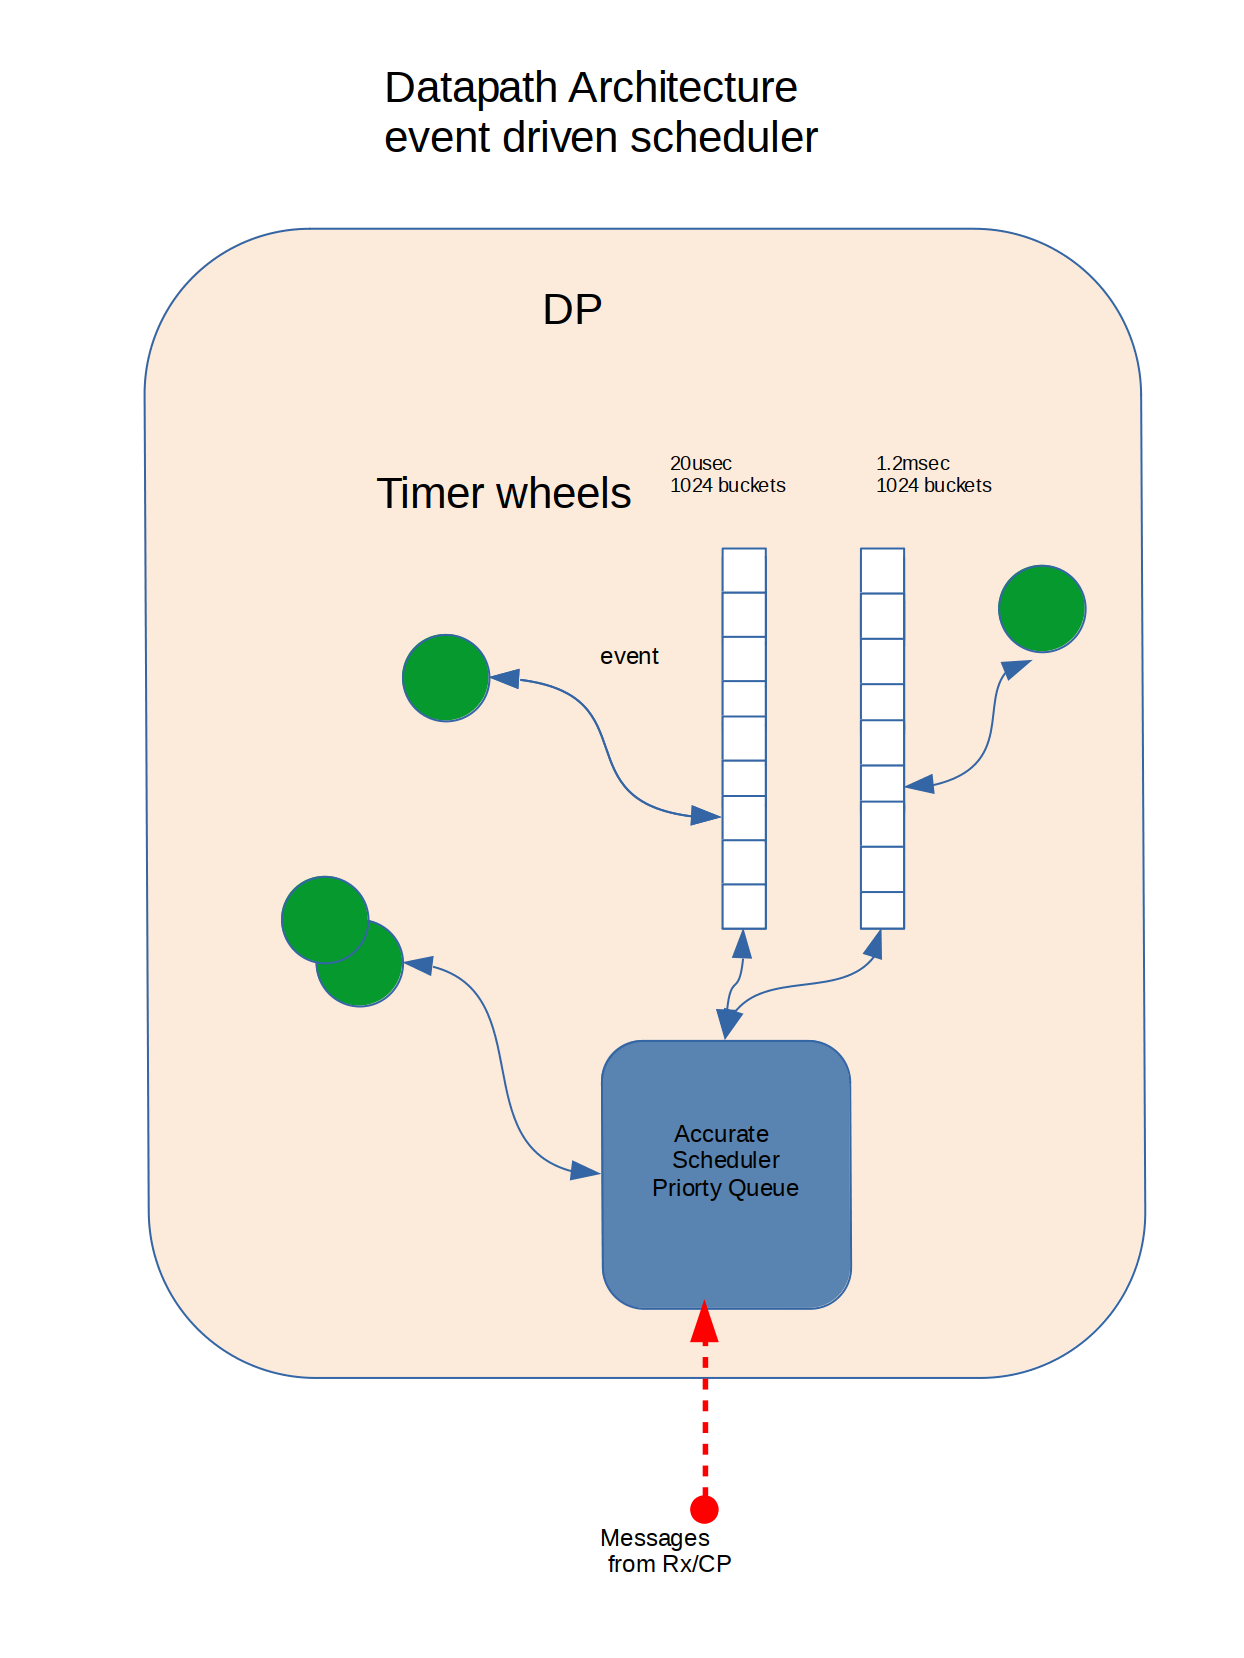
\includegraphics[width=0.4
  \textwidth, center]{trex_dp_sheduler.png}
  \caption{DP Scheduler}
  \label{fig:dp_schduler}
\end{figure}
  
Figure \ref{fig:dp_schduler} presents the schedulers in each DP thread. The priority queue is the low level scheduler that can schedule events in nsec resolution. On top of that there are two timer wheels for lower resolution events. The first has resolution of 20usec with 1024 buckets for maximum of 2msec time. 
the second timer wheel has resolution of 1msec with 1024 buckets maximum of 1sec. Each event in the second level is spread each 20usec tick to reduce processing spikes. 
DP transmit/receive messages from the share rings using events. 
This design gives linear scale with of performance about 4-20MPPS/core and 200gbps for one COGS server. 

\begin{figure}[h]
  \includegraphics[width=0.4
  \textwidth, center]{sfr_profile.png}
  \caption{emix}
  \label{fig:emix}
\end{figure}

From functionality point of view TRex has two main operation modes. Stateful and Stateless. Stateful is for testing L7 services that care about clients/flows/L7 application like DPI/NAT/Firewall, Figure \ref{fig:emix} is an example of mix of traffic that can be generated using this mode. 
Stateless is for testing Switch/Filters/ACL/Qos services and has no flow/client state

\section{Stateless mode}

\begin{figure}[h]
  \includegraphics[width=0.3
  \textwidth, center]{stateless_objects_02.png}
  \caption{Stateless objects}
  \label{fig:stlobjects}
\end{figure}


\begin{figure}[h]
  \includegraphics[width=0.4
  \textwidth, center]{stl_interleaving_01.png}
  \caption{Stateless profile example}
  \label{fig:stlhello}
\end{figure}



\section{Stateful mode}

// TBD this is an example 

\begin{itemize}
\item User space multi-threaded linux process TBD . DP cores (blue) can scale up
\item One thread per core, event driven, almost no sharing between the cores,no locks. This way multiplex many flows operation without context switch 
\item No syscall into kernel, driver are DPDK PMD for batching operations 
\item Each core has its own context, communication is via fast shared rings (DP$\rightarrow$CP, CP$\rightarrow$DP, Rx$\rightarrow$DP, RX$\rightarrow$CP)
\item Application emulation are via programable language that work in async API 
\begin{itemize}
    \item Start write buffer
    \item Continue write
    \item End Write
    \item Wait for buffer/timeout
    \item OnConnect/OnReset/OnClose
    \item Scale with the number of flows by having pull approach instead of push 
\end{itemize}
\end{itemize}

\begin{itemize}
\item Very low memory footprint with millions of flows (~1KB per flow)
\item 3-4MPPS/core almost linear scale with cores/flows. 
\item With average packet size of 600B (application application mix )  ~200gbps with x86 server with 2 sockets 
\end{itemize}


\section{Prepare Your Paper Before Styling}
Before you begin to format your paper, first write and save the content as a 
separate text file. Complete all content and organizational editing before 
formatting. Please note sections \ref{AA}--\ref{SCM} below for more information on 
proofreading, spelling and grammar.

Keep your text and graphic files separate until after the text has been 
formatted and styled. Do not number text heads---{\LaTeX} will do that 
for you.

\subsection{Abbreviations and Acronyms}\label{AA}
Define abbreviations and acronyms the first time they are used in the text, 
even after they have been defined in the abstract. Abbreviations such as 
IEEE, SI, MKS, CGS, ac, dc, and rms do not have to be defined. Do not use 
abbreviations in the title or heads unless they are unavoidable.

\subsection{Units}
\begin{itemize}
\item Use either SI (MKS) or CGS as primary units. (SI units are encouraged.) English units may be used as secondary units (in parentheses). An exception would be the use of English units as identifiers in trade, such as ``3.5-inch disk drive''.
\item Avoid combining SI and CGS units, such as current in amperes and magnetic field in oersteds. This often leads to confusion because equations do not balance dimensionally. If you must use mixed units, clearly state the units for each quantity that you use in an equation.
\item Do not mix complete spellings and abbreviations of units: ``Wb/m\textsuperscript{2}'' or ``webers per square meter'', not ``webers/m\textsuperscript{2}''. Spell out units when they appear in text: ``. . . a few henries'', not ``. . . a few H''.
\item Use a zero before decimal points: ``0.25'', not ``.25''. Use ``cm\textsuperscript{3}'', not ``cc''.)
\end{itemize}

\subsection{Equations}
Number equations consecutively. To make your 
equations more compact, you may use the solidus (~/~), the exp function, or 
appropriate exponents. Italicize Roman symbols for quantities and variables, 
but not Greek symbols. Use a long dash rather than a hyphen for a minus 
sign. Punctuate equations with commas or periods when they are part of a 
sentence, as in:
\begin{equation}
a+b=\gamma\label{eq}
\end{equation}

Be sure that the 
symbols in your equation have been defined before or immediately following 
the equation. Use ``\eqref{eq}'', not ``Eq.~\eqref{eq}'' or ``equation \eqref{eq}'', except at 
the beginning of a sentence: ``Equation \eqref{eq} is . . .''

\subsection{\LaTeX-Specific Advice}

Please use ``soft'' (e.g., \verb|\eqref{Eq}|) cross references instead
of ``hard'' references (e.g., \verb|(1)|). That will make it possible
to combine sections, add equations, or change the order of figures or
citations without having to go through the file line by line.

Please don't use the \verb|{eqnarray}| equation environment. Use
\verb|{align}| or \verb|{IEEEeqnarray}| instead. The \verb|{eqnarray}|
environment leaves unsightly spaces around relation symbols.

Please note that the \verb|{subequations}| environment in {\LaTeX}
will increment the main equation counter even when there are no
equation numbers displayed. If you forget that, you might write an
article in which the equation numbers skip from (17) to (20), causing
the copy editors to wonder if you've discovered a new method of
counting.

{\BibTeX} does not work by magic. It doesn't get the bibliographic
data from thin air but from .bib files. If you use {\BibTeX} to produce a
bibliography you must send the .bib files. 

{\LaTeX} can't read your mind. If you assign the same label to a
subsubsection and a table, you might find that Table I has been cross
referenced as Table IV-B3. 

{\LaTeX} does not have precognitive abilities. If you put a
\verb|\label| command before the command that updates the counter it's
supposed to be using, the label will pick up the last counter to be
cross referenced instead. In particular, a \verb|\label| command
should not go before the caption of a figure or a table.

Do not use \verb|\nonumber| inside the \verb|{array}| environment. It
will not stop equation numbers inside \verb|{array}| (there won't be
any anyway) and it might stop a wanted equation number in the
surrounding equation.

\subsection{Some Common Mistakes}\label{SCM}
\begin{itemize}
\item The word ``data'' is plural, not singular.
\item The subscript for the permeability of vacuum $\mu_{0}$, and other common scientific constants, is zero with subscript formatting, not a lowercase letter ``o''.
\item In American English, commas, semicolons, periods, question and exclamation marks are located within quotation marks only when a complete thought or name is cited, such as a title or full quotation. When quotation marks are used, instead of a bold or italic typeface, to highlight a word or phrase, punctuation should appear outside of the quotation marks. A parenthetical phrase or statement at the end of a sentence is punctuated outside of the closing parenthesis (like this). (A parenthetical sentence is punctuated within the parentheses.)
\item A graph within a graph is an ``inset'', not an ``insert''. The word alternatively is preferred to the word ``alternately'' (unless you really mean something that alternates).
\item Do not use the word ``essentially'' to mean ``approximately'' or ``effectively''.
\item In your paper title, if the words ``that uses'' can accurately replace the word ``using'', capitalize the ``u''; if not, keep using lower-cased.
\item Be aware of the different meanings of the homophones ``affect'' and ``effect'', ``complement'' and ``compliment'', ``discreet'' and ``discrete'', ``principal'' and ``principle''.
\item Do not confuse ``imply'' and ``infer''.
\item The prefix ``non'' is not a word; it should be joined to the word it modifies, usually without a hyphen.
\item There is no period after the ``et'' in the Latin abbreviation ``et al.''.
\item The abbreviation ``i.e.'' means ``that is'', and the abbreviation ``e.g.'' means ``for example''.
\end{itemize}
An excellent style manual for science writers is \cite{b7}.

\subsection{Authors and Affiliations}
\textbf{The class file is designed for, but not limited to, six authors.} A 
minimum of one author is required for all conference articles. Author names 
should be listed starting from left to right and then moving down to the 
next line. This is the author sequence that will be used in future citations 
and by indexing services. Names should not be listed in columns nor group by 
affiliation. Please keep your affiliations as succinct as possible (for 
example, do not differentiate among departments of the same organization).

\subsection{Identify the Headings}
Headings, or heads, are organizational devices that guide the reader through 
your paper. There are two types: component heads and text heads.

Component heads identify the different components of your paper and are not 
topically subordinate to each other. Examples include Acknowledgments and 
References and, for these, the correct style to use is ``Heading 5''. Use 
``figure caption'' for your Figure captions, and ``table head'' for your 
table title. Run-in heads, such as ``Abstract'', will require you to apply a 
style (in this case, italic) in addition to the style provided by the drop 
down menu to differentiate the head from the text.

Text heads organize the topics on a relational, hierarchical basis. For 
example, the paper title is the primary text head because all subsequent 
material relates and elaborates on this one topic. If there are two or more 
sub-topics, the next level head (uppercase Roman numerals) should be used 
and, conversely, if there are not at least two sub-topics, then no subheads 
should be introduced.

\subsection{Figures and Tables}
\paragraph{Positioning Figures and Tables} Place figures and tables at the top and 
bottom of columns. Avoid placing them in the middle of columns. Large 
figures and tables may span across both columns. Figure captions should be 
below the figures; table heads should appear above the tables. Insert 
figures and tables after they are cited in the text. Use the abbreviation 
 even at the beginning of a sentence.

\begin{table}[htbp]
\caption{Table Type Styles}
\begin{center}
\begin{tabular}{|c|c|c|c|}
\hline
\textbf{Table}&\multicolumn{3}{|c|}{\textbf{Table Column Head}} \\
\cline{2-4} 
\textbf{Head} & \textbf{\textit{Table column subhead}}& \textbf{\textit{Subhead}}& \textbf{\textit{Subhead}} \\
\hline
copy& More table copy$^{\mathrm{a}}$& &  \\
\hline
\multicolumn{4}{l}{$^{\mathrm{a}}$Sample of a Table footnote.}
\end{tabular}
\label{tab1}
\end{center}
\end{table}



Figure Labels: Use 8 point Times New Roman for Figure labels. Use words 
rather than symbols or abbreviations when writing Figure axis labels to 
avoid confusing the reader. As an example, write the quantity 
``Magnetization'', or ``Magnetization, M'', not just ``M''. If including 
units in the label, present them within parentheses. Do not label axes only 
with units. In the example, write ``Magnetization (A/m)'' or ``Magnetization 
\{A[m(1)]\}'', not just ``A/m''. Do not label axes with a ratio of 
quantities and units. For example, write ``Temperature (K)'', not 
``Temperature/K''.

\section*{Acknowledgment}

The preferred spelling of the word ``acknowledgment'' in America is without 
an ``e'' after the ``g''. Avoid the stilted expression ``one of us (R. B. 
G.) thanks $\ldots$''. Instead, try ``R. B. G. thanks$\ldots$''. Put sponsor 
acknowledgments in the unnumbered footnote on the first page.

\section*{References}

Please number citations consecutively within brackets \cite{b1}. The 
sentence punctuation follows the bracket \cite{b2}. Refer simply to the reference 
number, as in \cite{b3}---do not use ``Ref. \cite{b3}'' or ``reference \cite{b3}'' except at 
the beginning of a sentence: ``Reference \cite{b3} was the first $\ldots$''

Number footnotes separately in superscripts. Place the actual footnote at 
the bottom of the column in which it was cited. Do not put footnotes in the 
abstract or reference list. Use letters for table footnotes.

Unless there are six authors or more give all authors' names; do not use 
``et al.''. Papers that have not been published, even if they have been 
submitted for publication, should be cited as ``unpublished'' \cite{b4}. Papers 
that have been accepted for publication should be cited as ``in press'' \cite{b5}. 
Capitalize only the first word in a paper title, except for proper nouns and 
element symbols.

For papers published in translation journals, please give the English 
citation first, followed by the original foreign-language citation \cite{b6}.

\begin{thebibliography}{00}
\bibitem{b1} Cisco systems: ``TRex realistic traffic generator'',\\\texttt{https://trex-tgn.cisco.com/trex/doc/}
\bibitem{b2} Cisco systems, ``TRex Stateless'',,\\\texttt{https://trex-tgn.cisco.com/trex/doc/trex\\\_stateless.html}
\bibitem{b3} Cisco systems, ``TRex Stateful ASTF'',,\\\texttt{https://trex-tgn.cisco.com/trex/doc/trex\\\_astf.html}
\bibitem{b4} BIRD, Faculty of Math and Physics, Charles University Prague \\\texttt{https://bird.network.cz/}
\bibitem{b5} R. Nicole, ``Title of paper with only first word capitalized,'' J. Name Stand. Abbrev., in press.
\bibitem{b6} Y. Yorozu, M. Hirano, K. Oka, and Y. Tagawa, ``Electron spectroscopy studies on magneto-optical media and plastic substrate interface,'' IEEE Transl. J. Magn. Japan, vol. 2, pp. 740--741, August 1987 [Digests 9th Annual Conf. Magnetics Japan, p. 301, 1982].
\bibitem{b7} M. Young, The Technical Writer's Handbook. Mill Valley, CA: University Science, 1989.
\end{thebibliography}
\vspace{12pt}
\color{red}
IEEE conference templates contain guidance text for composing and formatting conference papers. Please ensure that all template text is removed from your conference paper prior to submission to the conference. Failure to remove the template text from your paper may result in your paper not being published.

\end{document}